\documentclass{beamer}

%\usetheme{Madrid}
%\usetheme{Boadilla}
%\usetheme{default}
%\usetheme{Warsaw}
%\usetheme{Bergen}
%\usetheme{Frankfurt}
\usetheme{Darmstadt}

\setbeamercolor{normal text}{fg=white}
\setbeamertemplate{background canvas}[vertical shading] [top=black!95,bottom=black!65]

\definecolor{mypurple}{RGB}{207,78,64}
\usecolortheme[named=mypurple]{structure}

\definecolor{myorange}{RGB}{255,235,190}
\beamerboxesdeclarecolorscheme{orange}{orange}{myorange}

\definecolor{commandcolor}{RGB}{111,195,165}

\setbeamertemplate{footline}[page number]
%\setbeamercovered{transparent}
\setbeamercovered{invisible}
\setbeamertemplate{navigation symbols}{}

%\usepackage{musixtex}
\usepackage{multimedia}
\usepackage{graphicx}
\usepackage[utf8]{inputenc}
%\usepackage[T1]{fontenc}
\usepackage[french]{babel} 
%\usepackage[all]{xy}
%\usepackage{multirow}
%\usepackage{lmodern}
\usepackage{subfigure}
%\usepackage{ulem}
\usepackage{url}
\usepackage{hyperref}
\usepackage{verbatim}
\usepackage{xspace}
\usepackage{color}
\usepackage{xcolor}
\usepackage{rotating}
\usepackage{multicol}
\usepackage[export]{adjustbox}
\usepackage{textpos}
\usepackage{listings}
\usepackage{fontawesome}


\definecolor{mypurple}{RGB}{207,78,64}
\usecolortheme[named=mypurple]{structure}

\definecolor{myorange}{RGB}{255,235,190}
\beamerboxesdeclarecolorscheme{orange}{orange}{myorange}

\definecolor{dgreen}{RGB}{0,125,0}

\usepackage{tikz}
\usetikzlibrary{trees}

\setbeamertemplate{caption}[numbered] 

\newcommand{\setframetitle}[1]{\begin{center}
    \huge \textbf{#1}
\end{center}}


%% --------------

\title{Docker}
\subtitle{Atelier d'aide à la programmation}
\author{L\'eo \textsc{Baudouin}}
\institute{
  {\url{baudouin.leo @ gmail.com}}
}
\date{13-14 juin 2024}

%% --------------

\begin{document}

\begin{frame}
  \titlepage
\end{frame}

\section{Introduction}
\subsection{}

\begin{frame}{Définition}


\begin{center}

\includegraphics[width=0.5\linewidth]{images/docker-logo}
\end{center}

\begin{block}{Wikipedia}
{\it 
«~Docker est un outil qui peut empaqueter une application et ses dépendances dans un conteneur isolé, qui pourra être exécuté sur n'importe quel serveur~».

Ceci permet d'étendre la flexibilité et la portabilité d’exécution d'une application, que ce soit sur la machine locale, un cloud privé ou public, une machine nue...}
\end{block}
\end{frame}


\begin{frame}[fragile]{Installer Docker}

\begin{block}{Installer et configurer}
\textcolor{cyan}{\verb?sudo apt-get install -y docker.io?}

\textcolor{cyan}{\verb?sudo groupadd docker?}

\textcolor{cyan}{\verb?sudo usermod -aG docker \$USER?}
\end{block}

\begin{block}{Docker for Windows}
\href{https://docs.docker.com/docker-for-windows/install/}{https://docs.docker.com/docker-for-windows/install/}
\end{block}

\end{frame}


\begin{frame}{Démarrer un conteneur}

\begin{block}{Télécharger une image}
\textcolor{cyan}{\verb?docker pull ubuntu:18.04?}
\end{block}

\begin{block}{Démarrer un conteneur}
\textcolor{cyan}{\verb?docker run --rm -it ubuntu:18.04?}
\end{block}

\end{frame}

\section{Images}
\subsection{Création}

\begin{frame}[fragile]{Créer une image pour \LaTeX}
\begin{block}{Dockerfile}
\begin{verbatim}
FROM ubuntu:18.04

RUN apt-get update
RUN apt-get upgrade -y 
RUN apt-get install -y texlive-full
\end{verbatim}
\end{block}
\end{frame}

\begin{frame}[fragile]{Créer une image pour Angular}
\begin{block}{Dockerfile}
\scriptsize
\begin{verbatim}
FROM ubuntu:18.04

RUN apt-get update && apt-get -y upgrade
RUN apt-get install -y npm

RUN npm install -g npm@latest
RUN npm install -g @angular/cli
RUN npm install --save-dev @angular-devkit/build-angular
RUN npm install --save-dev @angular/compiler-cli
RUN npm install --save-dev @angular/compiler
WORKDIR /sources

EXPOSE 8082
EXPOSE 4200

# ng serve --host 0.0.0.0
\end{verbatim}
\end{block}
\end{frame}



\begin{frame}[fragile]{Créer une image avec une interface}
\begin{block}{Dockerfile}
\scriptsize
\begin{verbatim}
FROM ubuntu:16.04

RUN apt-get update
RUN apt-get install -y x-window-system
RUN apt-get install -y binutils
RUN apt-get install -y mesa-utils
RUN apt-get install -y module-init-tools

ADD nvidia-driver.run /tmp/nvidia-driver.run
RUN sh /tmp/nvidia-driver.run -a -N --ui=none --no-kernel-module
RUN rm /tmp/nvidia-driver.run

RUN apt-get install -y nano

CMD /bin/bash

WORKDIR /sources
\end{verbatim}
\end{block}
\end{frame}



\section{Compose}
\subsection{}

\begin{frame}{docker-compose}
\begin{block}{Wikipedia}
{\it 
Docker \textbf{compose} est un outil très intéressant de gestion de package docker. Cet outil va lancer vos conteneurs et leurs éventuels liens à partir d'un fichier de configuration écrit en yaml.}
\end{block}
\end{frame}

\begin{frame}[fragile]{}
\begin{block}{\tiny docker-compose.yml}
\tiny
\begin{verbatim}
version: '3.3'
services:
   db:
     image: mysql:5.7
     volumes:
       - db_data:/var/lib/mysql
     restart: always
     environment:
       MYSQL_ROOT_PASSWORD: somewordpress
       MYSQL_DATABASE: wordpress
       MYSQL_USER: wordpress
       MYSQL_PASSWORD: wordpress
   wordpress:
     depends_on:
       - db
     image: wordpress:latest
     ports:
       - "8000:80"
     restart: always
     environment:
       WORDPRESS_DB_HOST: db:3306
       WORDPRESS_DB_USER: wordpress
       WORDPRESS_DB_PASSWORD: wordpress
   adminer:
     image: adminer
     depends_on:
       - db
     ports:
       - "8080:8080"
     restart: always
volumes:
    db_data:
\end{verbatim}
\end{block}
\end{frame}

\begin{frame}[fragile]{Démarrer / Arrêter}
\begin{block}{Gestion}
\textcolor{cyan}{\verb?docker-compose up [-d]?}

\textbf{-d} = run containers in the background
\newline

\textcolor{cyan}{\verb?docker-compose down?}
\end{block}
\end{frame}


\section{UI}
\subsection{}

\begin{frame}[fragile]{Gérer ses dockers}
\begin{block}{CLI}
\textcolor{cyan}{\verb?docker ps [-a]?}

\textcolor{cyan}{\verb?docker images?}
\end{block}

\begin{block}{Portainer}
\textcolor{cyan}{\verb?docker volume create portainer\_data?}

\textcolor{cyan}{\verb?docker run -d -p 9000:9000 --restart always -v /var/run/docker.sock:/var/run/docker.sock -v portainer\_data:/data portainer/portainer?}
\end{block}
\end{frame}


\begin{frame}[fragile]{Gérer ses dockers}
\begin{block}{Portainer}
\begin{center}
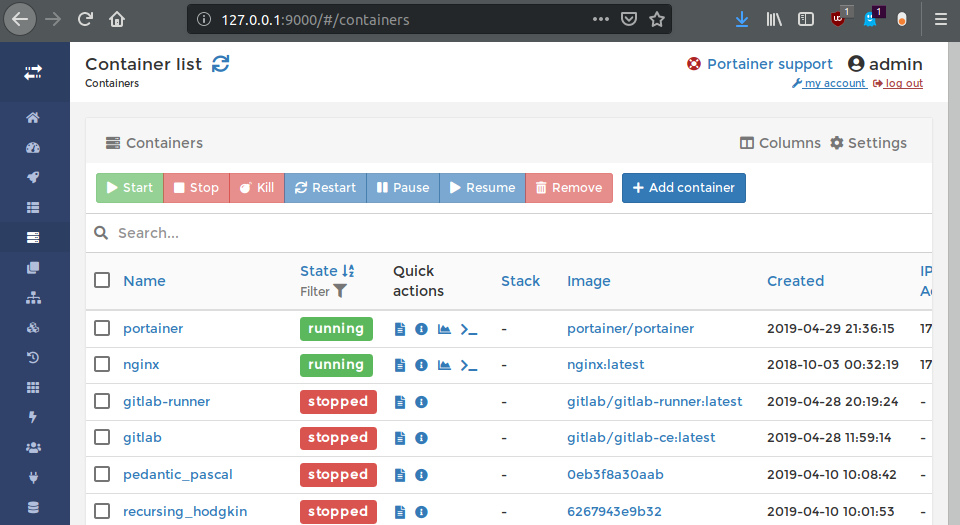
\includegraphics[width=1.0\linewidth]{images/portainer}
\end{center}
\end{block}
\end{frame}

%-------------------------------------------------------------------

\end{document} 
